\chapter{Reproducing the ADM Experiment}
\label{ch:reproduce_adm}

The following experiment was originally conducted in \cite{jazbec_generative_2025} to prove the applicability and usefulness of generative uncertainty in a large scale, state of the art diffusion model like \acs{ADM} against other baselines on the \acs{FPR} (FID, Precision and Recall) metrics. The idea here will be to prove that we can reproduce their experiment and get the same results. That will allow us to have the proper foundation to start extending their framework and conducting new experiments.

% Architecturally, ADM is built upon a modified U-Net backbone that incorporates multiple attention heads (with 64 channels per head) operating across several spatial resolutions ($32\times32$, $16\times16$, and $8\times8$). The network utilizes BigGAN-style residual blocks for upsampling and downsampling operations. Additionally, it employs Adaptive Group Normalization (AdaGN) layers, which integrate necessary conditioning by injecting timestep and class embeddings directly into the intermediate activations of the residual blocks.

% In the context of this thesis, ADM is used because it achieves exceptional visual fidelity and superior distribution coverage compared to traditional models like GANs, making it the standard for high-quality natural image generation[cite: 1368, 1371, 1588]. During our experiments, ADM is paired with deterministic DDIM sampling to efficiently evaluate complex datasets, such as high-resolution human hands[cite: 120, 121, 519]. This configuration provides an optimal, large-scale environment to observe and measure real-world mode interpolation, manifesting as out-of-distribution generative hallucinations (e.g., hands with additional or missing fingers)[cite: 521, 593].

\section{Setup}

\paragraph{Pipeline}
The idea here is to take the $\mathrm{M}+1=6$ ADM model weights including the base model and the 5 \acs{LLLA} sampled models, use a dataset of $12032$ noise samples through those $6$ models to get 12000 generated images for each model. 

The objective is to compare Generative Uncertainty to other baselines filtering metrics (Random, Rarity, Realism, \autoref{sec:inception_metrics}).
Once we have the $(\mathrm{M}+1) \times 12032$ images, we evaluate the baselines filtering metrics of each of the $12032$ images. We then filter out chunks of the $12032$ images with respect to each filtering metric (taking out the images than performs worse on those filtering metric first). The effect of that filtering is then measured on the \acs{FPR} metrics. 

% We measure the effect of filtering of by taking subset of $11000, 10000,..., 6000$ images and measuring the \acs{FPR} for each.

\paragraph{Implementation}
Thankfully, the original experiment from \cite{jazbec_generative_2025} was mostly already in their \texttt{github}. Although the realism baseline was already there, it was not fully implemented in the experiment's pipeline, the rarity baseline was not implemented at all. Some modifications were therefore made and are available in the \texttt{github} of this thesis.

\paragraph{Confidence Intervals}
It also worth noting that our reproduction of \parencite{jazbec_generative_2025} experiment did not include confidence intervals. Doing so would necessitate to run the very expensive\footnote{A full pass of the $\mathrm{M}+1=6$ models generating 12000 images each takes around 20 hours} image generation pipeline multiple times. 
We see on \autoref{fig:jazbec_exp} that the confidence intervals stay relatively small anyway and are not strictly required to see if a method performs better than another one. For this section in particular, we only needed to verify that our results were compatible with theirs.

\section{Experiment results}

We will first show the original figure from \parencite{jazbec_generative_2025} with \autoref{fig:jazbec_exp}

\begin{figure}[!htbp]
    \centering
    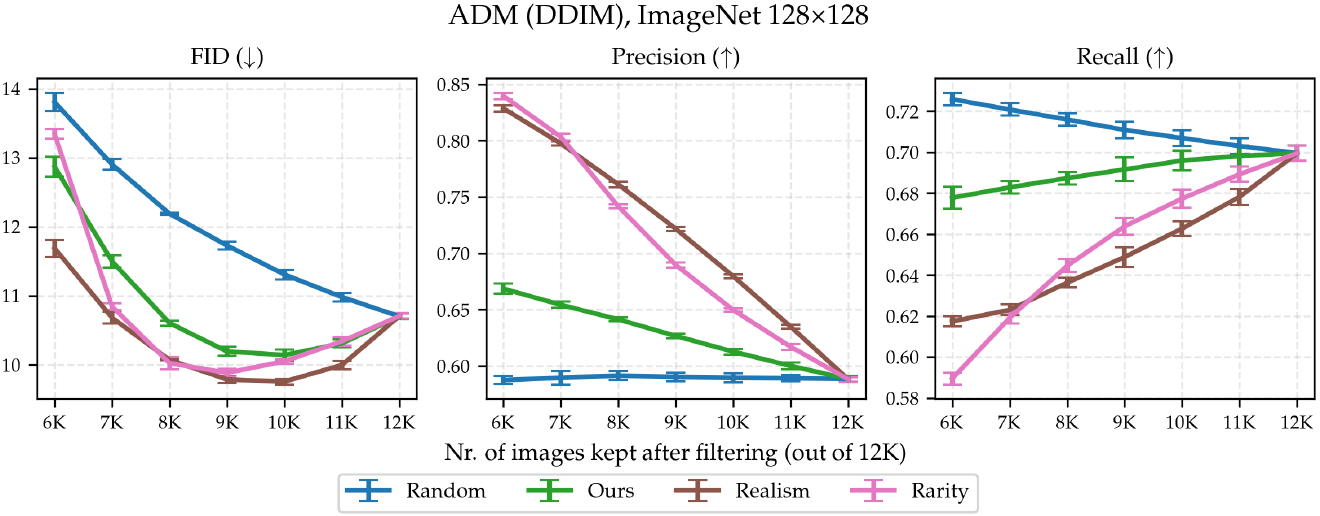
\includegraphics[width=0.9\linewidth]{figures/adm_experiment/jazbec_exp.png}
    \caption{Original experiment results from \cite{jazbec_generative_2025} appendix C.5. The unexpected steep rise in FID when reducing the number of images (even with the random baseline) is explained in \autoref{sub:problems_inception}}
    \label{fig:jazbec_exp}
\end{figure}

Then we take a look at our results with \autoref{fig:classifier_free}. We see that overall the behavior of all filtering baselines on all \acs{FPR} metrics are very similar to the original experiment. We can however see that Generative Uncertainty performed better on the FID metric in our experiment than it had in \parencite{jazbec_generative_2025}. This is unexpected since the generative uncertainty baseline is the only one that was already fully implemented in the original code and was not modified. 

Minor differences can be explained by the ImageNet dataset instance used.

\begin{figure}[!htbp]
    \centering
    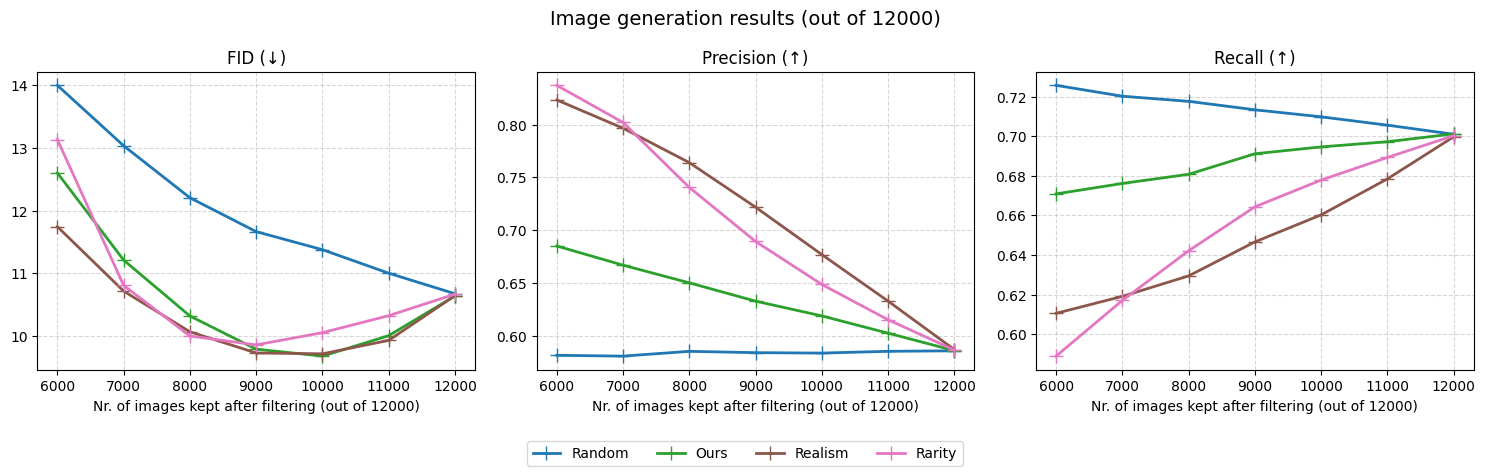
\includegraphics[width=0.99\linewidth]{figures/adm_experiment/classifier_free.png}
    \caption{Reproduced experiment results}
    \label{fig:classifier_free}
\end{figure}